\chapter{Versioning approaches}
\label{chap:versioning-approaches}

The service API can be versioned in multiple ways. One of the approaches is deployment of new version to new environment. This approach is widely used for code versioning not only for services. Other approach is specific for services. Multiple versions can coexist at the same time. Then there arises a question how a consumer can access the requested version of the service. The possibilities of access them is analyzed in Chapter \ref{chap:versionaccess}.


\section{New version - new environment approach}

The versioning is based on deploying a new version of \gls{api} to a new environment. The deployment process is identical to software deployment. Service changes are deployed on a new environment. %incrementing the API version number.

\subsection{Version identification}
When in an API with version \emph{v1} a change is done, implementation version number is incremented in minor digit. From the definition in Section \ref{subsec:versionid}, it is obvious that this is backward compatible change. The implementation than gains for example identifier \emph{1.1}. The services do not change their interface and their consumers are not affected. 
When there is a breaking change or there is a specified number of changes or amount of work done, API version increments and it is released to a new environment. 

The API version increase in major identifier to \emph{v2} because non-backward compatible changes were done. Consumers of services need to do required changes to use newer version of services. Than they call services using new environment. 
The API is usually marked by a major identifier so that \emph{API v1} or\emph{API v2} and so on.
The implementation of API is versioned using minor, path and revision identifiers. The implementation which is deployed on the server than can have a version for example \emph{1.0.0.0} or \emph{1.3.1.2}. The number increases depending on what kind of changes was done on the implementation.

Figure \ref{fig:version-identifying} shows an expamle of identification of version. Implementations of the version are identified by 4 digits. Last three of them are increasing within one version of service API. After a breaking change a new API version is created with incremented version number. 

\begin{figure}[htp] \centering{
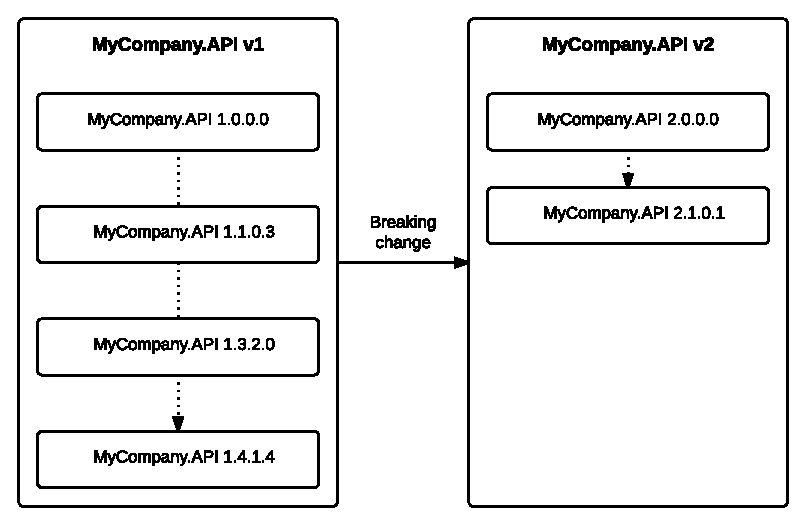
\includegraphics[width=8cm]{img/version-identifying.pdf}}
\caption{Incrementation of version identifiers}
\label{fig:version-identifying}
\end{figure} 


\subsection{Access to versions}
Consumers are always calling just one version of the API service. The one which is deployed to the targetted environment. They can switch she version of API only after deployment of new version on their production environment.

%\subsection{Advantages and disadvantages}
%Advantage of this approach is the access to API. He has accessible one version of API at the same time.

%The main disadvantage of this approach is the incapability of easily repair issues in a previous version of the API. When the API is in versions up to \emph{v3} in development environment and in versions \emph{v1} and \emph{v2} in production environment. When an error is found in production in \emph{v1} (Figure \ref{fig:bug-in-previous-version}) this bug is probably supposed to be present also in later versions \emph{v2} and \emph{v3}. Then the bug has to be fixed in all three versions and redeployed on servers which is usualy not a trivial operation.

%\begin{figure}[htp] \centering{
%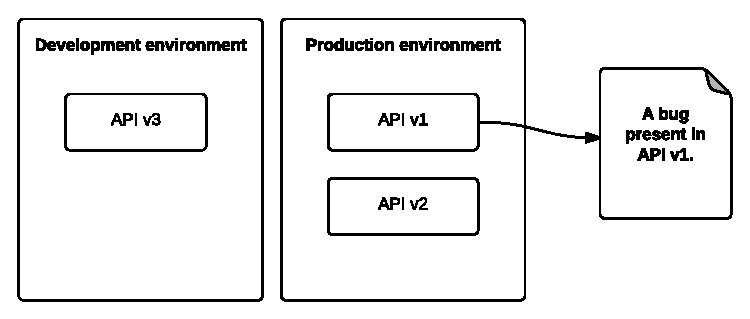
\includegraphics[width=11cm]{img/bug-in-previous-version.pdf}}
%\caption{An error found in one of the previous version}
%\label{fig:bug-in-previous-version}
%\end{figure} 


\section{Service interface versioning}

Another approach to versioning is more than one version of the service API running at the same time. This approach can be implemented using various principles. \emph{Service interface versioning} is the interpretation which will be further described and analyzed. It brings different principles of how to be accessed. Version access appraches will be explained in Chapter \ref{chap:versionaccess}.

This versioning approach allows to make changes to the API and release its new version without waiting for consumers to integrate the changes. All versions can run concurrently and be accessed by clients. When there are two coexistent versions of API, \emph{v1} and \emph{v2}, consumer has access to both of them. According to what he sent in the request he is directed to the correct version. Each of these versions can be on the same environment, or can be separated. This concept is invisible to  consumers.

%Each version has its own implementation and is distinguishably addressed.

%Versioning management of services requires the proper definition of following concepts \cite{website:versioning-in-soa}:
%what will be versioned and how, the life-cycle of the versions and the access to the version.
%\begin{enumerate}
 % \item Units of versioning
 % \item Service changes, constituting a new version
 % \item Service version life-cycle considerations
 % \item Version deployment/access approaches
%\end{enumerate}

\subsection{Units of versioning}
\label{sec:units}

The service layer of an application developed by a provider is an \emph{API} containing \emph{services}. Services contain \emph{methods (actions)} which allows to manipulate with the resources. The relationship between these entities is shown on Figure \ref{fig:service-layer-design}

\begin{figure}[htp] \centering{
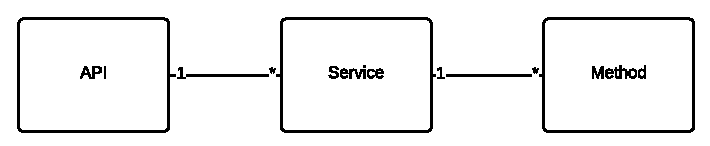
\includegraphics[width=11cm]{img/service-layer-design.pdf}}
\caption{Design of service layer}
\label{fig:service-layer-design}
\end{figure} 

Having this hierarchy there are three possibilities of what can be versioned in service interface. The granularity of versioning can be defined by the change which caused the creation of new version. If the change happens in method it is possible to version only the method. On the other hand, when a set of services are changed, whole API can be versioned. These are not rules but decisions. What to version should originate from the versioning strategy. 

Version is usually identified by one digit. This applies for each of the version unit. Than the architecture with different version of API, service and method can looks like the example on Figure \ref{fig:version-unit}. There is show the versioning on levels of API. The second part is a service versioning, \emph{Orders} service has two versions within an API. Third part show versioned method \emph{Get} which have \emph{v1} and \emph{v2} implementations.

\begin{figure}[htp] \centering{
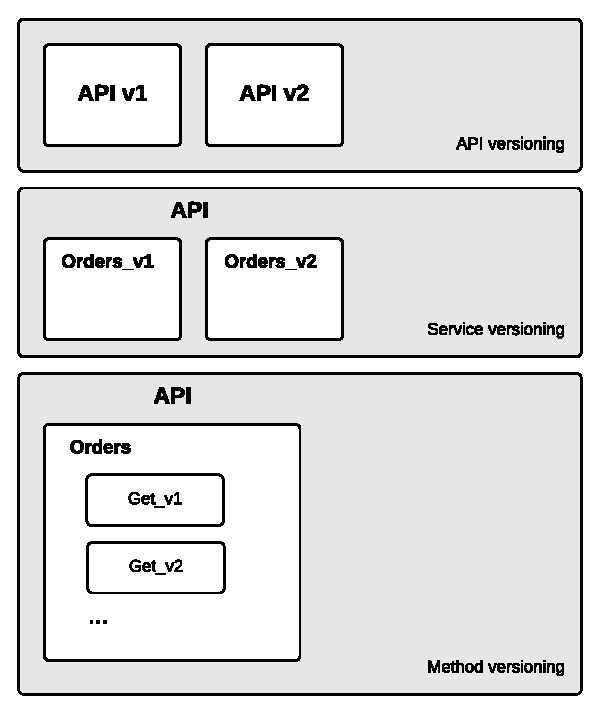
\includegraphics[width=9cm]{img/version-unit.pdf}}
\caption{Versioning units}
\label{fig:version-unit}
\end{figure} 

The three options can be combined. However cominantion of versioning of different granularity can result in complicated architecture of provided services.

\begin{description}
\item{API versioning} \\
The API containing all services can be versioned. Having a version \emph{v1} API is incremented to version \emph{v2}. This new version can be deployed on the same environment which was running the API v1. Consumers can access them both. Main disadvantage is the amount of redeployed code which contains mostly duplicated unchenged part of services. 
\item{Service versioning} \\
  A whole service is versioned with all its methods. Versioned service with version \emph{v1} is changed to \emph{v2}. It is still part of the API \emph{v1}, just the service version is incremented. When the new version on the service is deployed on environment both service versions can be accessed. 
\item{Method versioning} \\
  In most cases the change arises just in a method or a few methods of a service. It is not necessary to version the whole service, but there is an option to version just these methods. 
  
  Benefits of this approach are:
  
  \begin{enumerate}
    \item It minimize the amount of deployed code. Only changed methods are redeployed in a new version
    \item It allows immutable services names. There are only addition of new method or method deprecations.
  \end{enumerate}
  
  However it has this disadvantages:
  
  \begin{enumerate}
    \item It require more complex addressing schema. Instead od calling only service, consumers have to specify also the method and version of method which want to use.
    \item Versioned methods has to be deployed independently. More over every method has its own endpoint address.
  \end{enumerate}
\end{description}

%Other benefit of this versioning unit adding and removing of methods in a service. New method new can be added without any impact on existing consumer. Regarding the removal of a method, there is a deprecation concept. A method which has been for example replaced by new version can be signed as deprecated. A deprecated method takes part until there are still consumers which are using it. When all consumers stop to use it the method can be removed.\\


\subsection{Logic of service versioning}
There is a version of an API which is being used in production. A breaking change needs to be applied and new API version is created. Both versions can be deployed into production, it is not mandatory for both of them to be on the same environment. Consumer can continue to use the old version, he can switch the version integrating the changes whenever. It is needed to be clear in advance where the version will be placed and how will it be accessed.

Depending on the principle of accessing the version, it can be said explicitly in endpoint address (URL) which version of API, service or method is called. The request is directly roated to requested version. The other approach is to have the same endpoint address for each version of the versioned unit. Routing passes through an intermedia which resolves the correct version. Decision is based on one of the parameters send in request. Option of accessing the version will be described in Chapter \ref{chap:versionaccess}.

/todo
parallel development
version lifecycle, how long to maintain the version

\subsection{Advantages and disadvantages}
The advantage is the version access at any time after deployment in production, the process in not dependent on consumers integration. The other very significant advantage is the fixing of failures, ???
On customer site the disadvantage is the forcing to add the version identification in the requests, he has to change it everytime he change the version of API or its subunits. For provider it is needed to implement a logic of access different versions.
/TODO
